\begin{problem}{DP | LC2361 | Minimum Costs Using the Train Line
    }
    LC2361

    A train line going through a city has two routes, the regular route and the express route. Both routes go through the same n + 1 stops labeled from 0 to n. Initially, you start on the regular route at stop 0.

You are given two 1-indexed integer arrays regular and express, both of length n. regular[i] describes the cost it takes to go from stop i - 1 to stop i using the regular route, and express[i] describes the cost it takes to go from stop i - 1 to stop i using the express route.

You are also given an integer expressCost which represents the cost to transfer from the regular route to the express route.

Note that:

There is no cost to transfer from the express route back to the regular route.
You pay expressCost every time you transfer from the regular route to the express route.
There is no extra cost to stay on the express route.
Return a 1-indexed array costs of length n, where costs[i] is the minimum cost to reach stop i from stop 0.

Note that a stop can be counted as reached from either route.

\footnote{html present in question-html folder}
\end{problem}

\begin{solution}[Dynamic Programming | ways at idx]
    This is standard variation of ways at idx.
    As usual if the problemm was to have compute the optmal cost to reach start to end, then this problem could be solved via (a) left to right (\verb|f(0,_)|) or (b) via right to left(\verb|f(size-1,_|).

    But now this question emphaisis to use \verb|f(size-1,_)| as we need to compute cost at each step.

    To do this, we will simply find out the ways to reach idx and will implement them in code with ontrack restriction.

    \begin{marginfigure}
        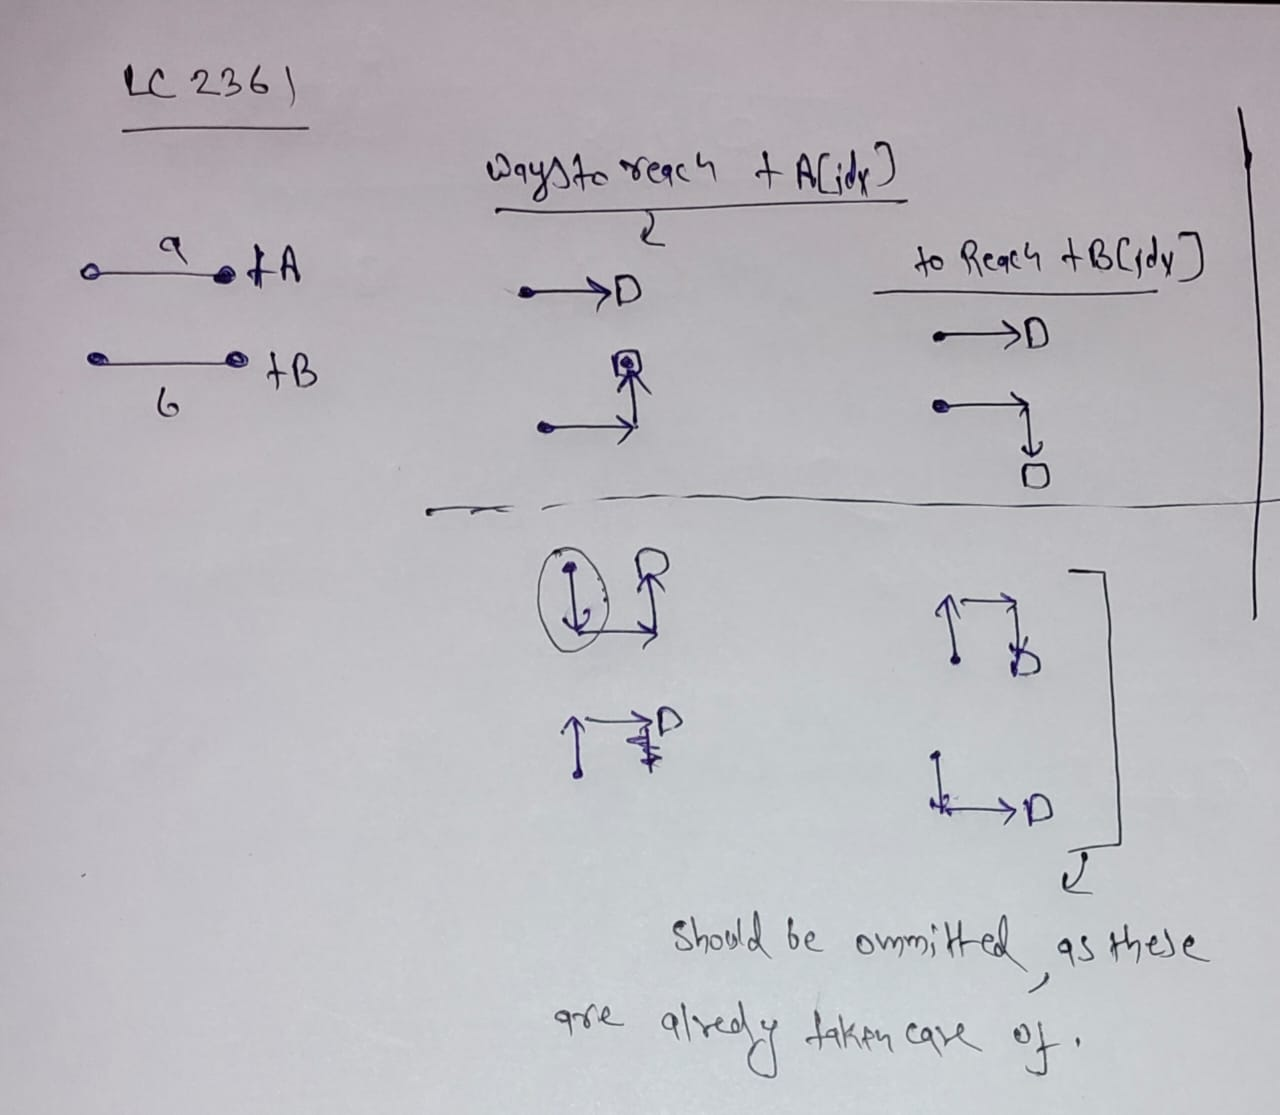
\includegraphics[width=\marginparwidth]{res/LC2361.jpg}
    \end{marginfigure}

    \begin{fullwidth}
    \begin{code3}[right to left memoization]
    /* ontrack is, on which track we are requessted to land the train at idx*/
    lli findAnsFive(int idx,int ontrack,vector<int>& tA, vector<int>& tB, int tcc)
    {
        if(idx<0) return ontrack == 0?0:tcc;
        
        lli &mans = mem[idx][ontrack];
        if(mans != -1) return mans;
        
        /* options at idx, you can think as other option also: reach via tA, reach via tB*/
        lli val1; //reach via tA
        lli val2; //reach via tB
        
        lli t1 = findAnsFive(idx-1,0,tA,tB,tcc); //arrive from tA (cost to reach tA[idx-1] on platform tA)
        lli t2 = findAnsFive(idx-1,1,tA,tB,tcc);  //arrive from tB
        
        if(ontrack == 0) //regular track
        {
            val1 = t1 + tA[idx]; //AA
            val2 = t2 + tB[idx]+0; //BA
        }
        else
        {
            val1 = t1 + tA[idx] + tcc; //AB
            val2 = t2 + tB[idx]; //BB
            
        }
        
        //   printf("[%d,%d]:(%d,%d)\n",idx,ontrack,val1,val2);
        return mans = min(val1,val2);    
    }

    //findAnsFive(tA.size()-1,0,tA,tB,expressCost);
    //findAnsFive(tA.size()-1,1,tA,tB,expressCost);
    \end{code3}


    \begin{code3}[left to right memoization]
    /* code not submitted*/
    /* ptrack is from which track train is coming*/
    lli findAns(int idx,int ptrack,vector<int>& tA,vector<int>&tB,const int trackChangeCost)
    {
        if(idx >= tA.size()) return 0;
        
        lli &mans = mem[idx][ptrack];
        if(mans != -1) return mans;
        
        /* all options to reach this idx*/
        lli val1; //continue one same track
        lli val2; //change track
        
        /* or: continue via trackA, continue via trackB*/
        
        if(ptrack == 0) //train was previously at tA
        {
            val1 =  tA[idx] + findAns(idx+1,0,tA,tB,trackChangeCost); 
            val2 =  tB[idx] + trackChangeCost
                            + findAns(idx+1,1,tA,tB,trackChangeCost); 
        }
        else //train was previous on tB (on express route)
        {
            val1 =  tB[idx] + findAns(idx+1,1,tA,tB,trackChangeCost); 
            val2 =  tA[idx] + findAns(idx+1,0,tA,tB,trackChangeCost);
        }
        
        // printf("[%d,%d]:(%d,%d)\n",idx,ptrack,val1,val2);
        return  mans = min(val1,val2);
    }

       //return findAns(0,0,tA,tB,expressCost) 
    \end{code3}
\end{fullwidth}

\end{solution}